% !TeX root = RJwrapper.tex
\title{\pkg{cvcqv}: A Package for Estimation of Relative Variability}
\author{by Maani Beigy}

\maketitle

\abstract{%
Coefficient of variation (\emph{cv}) and coefficient of quartile variation (\emph{cqv}) are widely used measures of relative dispersion which play descriptive and inferential roles (\emph{e.g.,} reliability analysis, quality control, inequality measurement, and anomaly detection) in various fields such as biological and medical sciences, economics, actuarial sciences, etc. Since \emph{cv} and \emph{cqv} are unit-free, they are useful for comparing data from different distributions, data from different scales, or widely different means. However, to avoid their common misuses, confidence intervals (\emph{CI}) are required. The \textbf{cvcqv} package provides a home for such tools. To our knowledge, the new \code{R} package \textbf{cvcqv} is the first \code{R} implementation of \textbf{cqv} as a robust variability measure, with almost all available methods for \emph{CI} of \emph{cv} and \emph{cqv}. This paper elucidates this versatile functionality using reproducible examples on real datasets. Also, the new insights that \textbf{cvcqv}, alongside other \code{R} packages, brings into data science will be discussed. 
}

\section{Introduction}

Researchers and practitioners in various fields use the coefficient of variation  (\emph{cv}) as a measure of relative variability \citep{Panichkitkosolkul_2013, Payton_1996}. \emph{cv} is calculated as the ratio of the sample standard deviation (\emph{sd}) to the sample mean ($\overline{x}$). However, \emph{cv} is often misleading for variables with non-ratio scales \citep{Payton_1996}, for homoscedastic data, and for variables without different magnitudes or units \citep{Shechtman_2013}.

Robust statistical measurements such as coefficient of quartile variation (\emph{cqv}) are better alternatives in non-normal distributions \citep{Altunkaynak_2018}:
$$
cqv = \biggl(\frac{q_3-q_1}{q_3+q_1}\biggr)\times100
$$
where $q_3$ and $q_1$ are the sample third quartile (\emph{i.e.,} $75^{th}$ percentile) and first quartile (\emph{i.e.,} $25^{th}$ percentile), respectively.

Almost always, we calculate \emph{cv} and \emph{cqv} from samples but the final objective is to generalize them as the populations' parameters \citep{Albatineh:2014}. For example, one may be interested in comparing the variabilities of the time-varying measurements of a variable to detect anomalies such as extreme behaviors of customers or institutes (as in actuarial sciences). Or someone might inquire into whether a laboratory test or technique has sufficient inter-assay and intra-assay reliability \citep{Panichkitkosolkul_2013, Payton_1996}. In such scenarios, variabilities calculated from samples are often biased and misleading \citep{sorensen_2002, Payton_1996}. Therefore, various confidence intervals (\emph{CI}) have been introduced to correctly estimate the relative variability. 

This paper sets out to demonstrate the versatility of \CRANpkg{cvcqv} package \citep{Beigy_a_2019} in a variety of data science tasks related to variability measurement. \code{R} \citep{R} provides a strong asset for progress in this direction because it already contains functionality used in a variety of packages like \CRANpkg{DescTools}, \CRANpkg{MBESS}, \CRANpkg{goeveg}, and \CRANpkg{sjstats}. However, robust variability measures such as \emph{cqv} has been missing in \code{R} for a long time. Moreover, the implementations of \emph{CI} for \emph{cv} have been limited to one or two methods. Lack of functions for the rigorous methods of calculation of \emph{CI} for \emph{cv} and \emph{cqv}, though available in the statistical literature, was a major motivation to develop this package and explain its versatile functionality in this paper.  

\section{Package structure and functionality}

The package can be installed and loaded as follows (see the package’s \href{https://github.com/MaaniBeigy/cvcqv/blob/master/README.md}{README} for dependencies and access to development versions):

\begin{example}
install.packages("cvcqv")
\end{example}

\begin{example}
library(cvcqv)
\end{example}

\textbf{cvcqv} depends on \CRANpkg{dplyr} \citep{wickham_2019} for using \code{nth()} function and imports \CRANpkg{R6} \citep{chang_2019} for \code{"R6"} classes, \CRANpkg{SciViews} \citep{grosjean_2018} for \code{ln()} function, \CRANpkg{boot} \citep{canty_2019} for bootstrapping methods, and \CRANpkg{MBESS} \citep{kelley_2018} for noncentral distributions.

\subsection{Core functions and classes}\label{core-functions-and-classes}

The functionality of the package is developed as both simple functions and \code{"R6"} classes, for sake of versatility, portability and efficiency:

\begin{itemize}
\tightlist
\item
  The R6 class \code{"SampleQuantiles"} to produce the sample quantiles corresponding to the given probabilities. It uses \href{https://stat.ethz.ch/R-manual/R-devel/library/stats/html/quantile.html}{quantile} function from the built-in \code{R} package \strong{stats}, but provides an \code{"R6"} interface to be inherited for other classes.
\item
  The R6 class \code{"BootCoefVar"} produces the bootstrap resampling for the \emph{cv}. It uses \href{https://stat.ethz.ch/R-manual/R-patched/library/boot/html/boot.ci.html}{boot.ci} function from \CRANpkg{boot}, but provides an \code{"R6"} interface to be inherited for child classes.
\item
  The R6 class \code{"BootCoefQuartVar"} produces the bootstrap resampling for the \emph{cqv}. It uses \href{https://stat.ethz.ch/R-manual/R-patched/library/boot/html/boot.html}{boot} and \href{https://stat.ethz.ch/R-manual/R-patched/library/boot/html/boot.ci.html}{boot.ci} functions from \CRANpkg{boot}, but provides an \code{"R6"} interface to be inherited for child classes.
\item
  The R6 class \code{"CoefVar"} calculates the sample \emph{cv}.
\item
  The R6 class \code{"CoefQuartVar"} calculates the sample \emph{cqv}.
\item
  The R6 class \code{"CoefVarCI"} calculates \emph{CI} for \emph{cv}.
\item
  The R6 class \code{"CoefQuartVarCI"} calculates \emph{CI} for \emph{cqv}.
\item
  The function \code{cv\_versatile} calculates \emph{cv} and its various \emph{CIs}.
\item
  The function \code{cqv\_versatile} calculates \emph{cqv} and its various \emph{CIs}.
\end{itemize}

\subsection{R6 Objects Tree}
\begin{verbatim}
SampleQuantiles
      ├─── BootCoefVar
      │    └────────── CoefVar
      │                  └────────── CoefVarCI
      │  
      └─── BootCoefQuartVar
           └────────── CoefQuartVar
                         └────────── CoefQuartVarCI
\end{verbatim}

\subsection{Confidence Interval Methods}

There are various methods for the calculation of \emph{CI} for \emph{cv} and \emph{cqv}, which have been implemented in \textbf{cvcqv} package:

\setlength\tabcolsep{2pt}
\begin{longtable}{|c|c|}
\caption{
Methods for calculation of \emph{CI} for \emph{cv} and \emph{cqv}
}\\
\hline
\textbf{cv} & \textbf{cqv} \\
\hline
\endfirsthead
\multicolumn{2}{c}%
{\tablename\ \thetable\ -- \textit{Continued from previous page}} \\
\hline
\textbf{cv} & \textbf{cqv} \\
\hline
\endhead
\hline \multicolumn{2}{r}{\textit{Continued on next page}} \\
\endfoot
\hline
\endlastfoot
"kelley" (\citeyear{kelley_2018, Kelley_2007}) & "bonett" (\citeyear{Bonett_2006}) \\ "mckay" (\citeyear{McKay_1932}) & "norm" (\citeyear{Altunkaynak_2018}) \\ "miller" (\citeyear{EdwardMiller_1991}) & "basic" (\citeyear{Altunkaynak_2018}) \\ "vangel" (\citeyear{Vangel_1996}) & "perc" (\citeyear{Altunkaynak_2018}) \\ "mahmoudvand\_hassani" (\citeyear{Mahmoudvand_2009}) & "bca" (\citeyear{Altunkaynak_2018}) \\ "equal\_tailed" (\citeyear{Panichkitkosolkul_2013}) &  \\ "shortest\_length" (\citeyear{Panichkitkosolkul_2013}) &  \\ "normal\_approximation" (\citeyear{Panichkitkosolkul_2013}) &  \\ "norm" (\citeyear{canty_2019, davison_1997}) &  \\ "basic" (\citeyear{canty_2019, davison_1997}) &  \\ "perc" (\citeyear{canty_2019, davison_1997}) &  \\ "bca" (\citeyear{canty_2019, davison_1997}) &  \\
\end{longtable} 

For more statistical details on these methods, read the vignettes provided for \href{https://cran.r-project.org/web/packages/cvcqv/vignettes/cv_versatile.html}{\code{cv}} and \href{https://cran.r-project.org/web/packages/cvcqv/vignettes/cqv_versatile.html}{\code{cqv}} \citep{Beigy_a_2019}.

\section{Solutions for real-world problems}

This section contains examples on real-world data science problems: 


\subsection{Consistency or Reliability of Measurements}

Instruments and measurements have to be not only valid but also reliable. 
Reliability is defined as the extent to which they measure the variables consistently \citep{Shechtman_2013}. Reliability may also be called as consistency, repeatability, reproducibility, stability, and precision \citep{Shechtman_2013}.

The \emph{cv} and \emph{cqv} can be used as indicators of reliability because they assesses the stability of measurements across repeated tests. An advantage of dimensionless measures such as \emph{cv} and \emph{cqv} is that they allow us to make direct comparisons between the measurements regardless of the scale or calibration. Hence, they enable us to compare reliability among instruments and assays \citep{Shechtman_2013, hopkins_2000}.

In terms of assessing the reliability of measurements, the interesting questions  \href{https://stats.stackexchange.com/questions/318044/how-to-measure-consistency-of-measurement-over-time}{How to measure consistency of measurement over time} and  \href{https://stats.stackexchange.com/questions/398462/how-to-measure-the-consistency-of-improvement-on-different-conditions}{How to measure the consistency of improvement on different conditions?} on Cross Validated  \href{https://stats.stackexchange.com/}{community statistics}, properly address such problem \citep{tach_2017, Ida_2019}. Inspired by them, a sample \code{data.frame} named \code{wine.csv} for testing the quality of \strong{five different type of wines} by \strong{three experts} was created. A small chunk of the \code{data.frame} is:

\begin{example}
     expert    measurement Wine_1 Wine_2 Wine_3 Wine_4 Wine_5
1    expert_a  2019-01-01   0.70   0.60   0.30   0.10   0.80
2    expert_a  2019-01-02   0.60   0.70   0.40   0.20   0.80
3    expert_a  2019-01-03   0.65   0.65   0.35   0.15   0.80
44   expert_b  2019-01-04   0.90   0.10   0.90   0.10   0.90
45   expert_b  2019-01-05   0.20   0.12   0.21   0.31   0.21
46   expert_b  2019-01-06   0.80   0.56   0.79   0.89   0.69
115  expert_c  2019-02-04   0.43   0.24   0.15   0.68   0.92
116  expert_c  2019-02-05   0.42   0.32   0.16   0.69   0.91
117  expert_c  2019-02-06   0.41   0.31   0.15   0.70   0.90
\end{example}

Then, we prepare the data using the \CRANpkg{tidyverse} \citep{Wickham_2017} packages. We need the \code{wine} \code{data.frame} in the long format:
\begin{example}
library(tidyverse)
wine_gather %>% gather(
  key = "wines",
  value = "score",
  Wine_1:Wine_5, -measurement
)
\end{example}
Then, we test the normality of \code{scores} variable:
\begin{example}
shapiro.test(wine$score)
	Shapiro-Wilk normality test

data:  wine_gather$score
W = 0.89857, p-value < 2.2e-16
\end{example}

Because of the non-normal distribution of the \code{scores} variable, we calculate the \emph{cqv} with \emph{Bootstrap percentile 95\% CI} using \CRANpkg{cvcqv} \code{R6} class \code{CoefQuartVarCI} with \code{perc\_ci} method:

\begin{example}
library(cvcqv)
wine_gather %>% group_by(expert, wines) %>% summarise(
  cqv_est = cvcqv::CoefQuartVarCI$new(
    x = score, na.rm = TRUE, alpha = 0.05, R = 100, digits = 3,
  )$perc_ci()$statistics$est,
  cqv_lower = cvcqv::CoefQuartVarCI$new(
    x = score, na.rm = TRUE, alpha = 0.05, R = 100, digits = 3,
  )$perc_ci()$statistics$lower,
  cqv_upper = cvcqv::CoefQuartVarCI$new(
    x = score, na.rm = TRUE, alpha = 0.05, R = 100, digits = 3,
  )$perc_ci()$statistics$upper
)

   expert   wines  cqv_est cqv_lower cqv_upper
 1 expert_a Wine_1    5.58     3.33       6.15
 2 expert_a Wine_2    3.3      2.33       4.70
 3 expert_a Wine_3    6.02     4.22       8.01
 4 expert_a Wine_4   12.5      7.06      18.8 
 5 expert_a Wine_5    1.38     0.621      2.5 
 6 expert_b Wine_1   70.3     47.1       75.6 
 7 expert_b Wine_2   66.0     52.9       69.1 
 8 expert_b Wine_3   58       55.3       58.4 
 9 expert_b Wine_4   45.8     31.2       70.8 
10 expert_b Wine_5   49.9     13.3       53.6 
11 expert_c Wine_1   30.1     18.3       53.7 
12 expert_c Wine_2   49.6     10.7       52.3 
13 expert_c Wine_3   70.9     39.2       72.4 
14 expert_c Wine_4   14.5      4.74      15.9 
15 expert_c Wine_5   70.7      9.61      76.0 
\end{example}

As you see in figure~\ref{figure:fig1}, only the \strong{expert\_a} shows consistent measurements for various wines over time; because large measurements with \emph{cqv} or \emph{cv} values (here higher than 10\%) are generally considered non-reliable \citep{Beigy_b_2019}:

\begin{figure}[htbp]
  \centering
  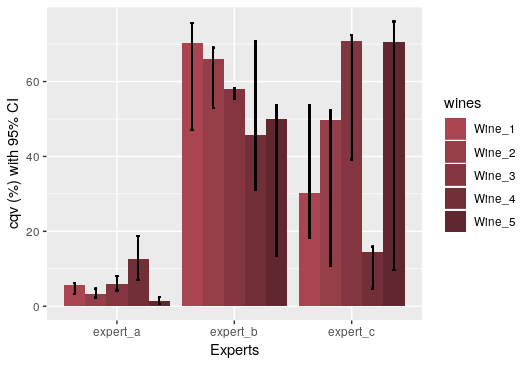
\includegraphics[width=0.5\linewidth]{fig1}
  \caption{The consistency of experts' scores on the different wine types over time}
  \label{figure:fig1}
\end{figure}

\subsection{Detection of Outliers and Anomalies}

The \emph{cv} and \emph{cqv} play direct and indirect roles to detect outliers \citep{zhou_2014} and anomalies \citep{fathnia_2018}. Detecting variables or measurements with high \emph{cv} or \emph{cqv} migth be helpful before employing anomaly detection techniques. An example is provided here based on the question of \citet{Ida_2019}, investigating the speed improvement of various cases (codes in \code{anomaly.R} \href{https://github.com/MaaniBeigy/cvcqv/blob/master/docs/articles/anomaly.R}{file}). Let us use the \code{data.frame} called \code{speed\_tbl\_df}:

\begin{example}
head(speed_tbl_df)
        date case speed
1 2019-01-01    A   1.2
2 2019-01-02    A   1.3
3 2019-01-03    A   1.1
4 2019-01-04    A   1.1
5 2019-01-05    A   1.5
6 2019-01-01    B   1.2
\end{example}

We calculate \emph{cv} and \emph{cqv} with \emph{Basic bootstrap 95\% CI} for cases A, B, and C: 

\begin{example}
head(speed_tbl_df)
cqv_speed_A <- cvcqv::CoefQuartVarCI$new(
  x = subset(speed_tbl_df, case == "A")$speed, 
  na.rm = TRUE, 
  digits = 3, 
  R = 1000, 
  alpha = 0.05
  )$basic_ci()

cv_speed_A <- cvcqv::CoefVarCI$new(
  x = subset(speed_tbl_df, case == "A")$speed, 
  na.rm = TRUE, 
  digits = 3, 
  R = 1000, 
  alpha = 0.05
)$basic_ci() 

# do the same for the remaining cases B and C.Then, collect them all in one df:
cvcqv_speed <- dplyr::bind_rows(list(
  cqv_speed_A$statistics,
  cqv_speed_B$statistics,
  cqv_speed_C$statistics,
  cv_speed_A$statistics,
  cv_speed_B$statistics,
  cv_speed_C$statistics
))
attr(cvcqv_speed, "row.names") <- c(
  "cqv_A", "cqv_B", "cqv_C", "cv_A", "cv_B", "cv_C"
  )
cvcqv_speed
          est  lower   upper
cqv_A   8.333  1.282  16.667
cqv_B  92.308 86.791 184.615
cqv_C  42.857 28.852  85.714
cv_A   13.495  9.627  22.996
cv_B  133.997 80.843 214.743
cv_C   54.696 36.741  87.258
\end{example}

As I explained in the question on Cross Validated \citep{Beigy_c_2019}, case A shows minimal variability ($ \approx 8\% $); case B shows severe variation ($ \approx 92\% $), and case C shows moderate variation ($ \approx 43\% $). In cases with severe variation, it is more probable to find anomalies. Here, \CRANpkg{anomalize} \citep{Dancho_2018} package may be helpful:

\begin{example}
anomalize::anomalize(speed_tbl_df, speed, method = "iqr", alpha = 0.05)
# A tibble: 15 x 6
   date       case  speed speed_l1 speed_l2 anomaly
   <date>     <fct> <dbl>    <dbl>    <dbl> <chr>  
 1 2019-01-01 A       1.2    -5.90     10.5 No     
 2 2019-01-02 A       1.3    -5.90     10.5 No     
 3 2019-01-03 A       1.1    -5.90     10.5 No     
 4 2019-01-04 A       1.1    -5.90     10.5 No     
 5 2019-01-05 A       1.5    -5.90     10.5 No     
 6 2019-01-01 B       1.2    -5.90     10.5 No     
 7 2019-01-02 B       1.1    -5.90     10.5 No     
 8 2019-01-03 B      20      -5.90     10.5 Yes    
 9 2019-01-04 B      30      -5.90     10.5 Yes    
10 2019-01-05 B     100      -5.90     10.5 Yes    
11 2019-01-01 C       1.2    -5.90     10.5 No     
12 2019-01-02 C       1.1    -5.90     10.5 No     
13 2019-01-03 C       2      -5.90     10.5 No     
14 2019-01-04 C       3      -5.90     10.5 No     
15 2019-01-05 C       4      -5.90     10.5 No    
\end{example}

As you can see in the anomaly column of the result, the speed improvements of \code{"20, 30, 100"} of case B (the one with severe variability based on \emph{cqv}) are anomalies/outliers. 

\bibliography{RJreferences}

\address{%  
  Maani Beigy\\
  Department of Epidemiology and Biostatistics\\
  School of Public Health\\
  Tehran University of Medical Sciences\\
  Tehran\\
  Iran\\
  ORCiD: 0000-0003-2963-3533\\
  \email{manibeygi@gmail.com}\\
  \email{m-beigy@alumnus.tums.ac.ir}
}